% This file contains the content for a main section
\numberedformat
%% Modify below this line %%

\clearpage
\chapter{Recommended Workflows}
\label{ch:rec-workflows}
This section is intended to outline the recommended usage of ACES Output Transforms as they apply to common workflows applicable to feature motion picture and episodic television production.

%%%%%%%%%% Workflow %%%%%%%%%% 
\section{Feature Film Workflows}

\subsection{Production and Mastering -- SDR On-Set and Digital Intermediate}

\subsubsection{Summary}
It is common in the production of digital feature films to monitor the output of the camera on-set to check for framing, exposure, and often to create looks.  Looks are often created on-set or near-set using an on-set grading system with the result being a series of ASC-CDL values that are passed to digital intermediate (DI) mastering facility as a starting point for final grading.  In order to insure looks are set and communicated from on-set to the DI master facility as intended, it's important that the correct Output Transforms be used in each location.  The following is a recommendation for the usage of Output transforms for a common on-set to digital intermediate workflow.

\subsubsection{Workflow}
The complete workflow from camera to post is beyond the scope of this document, but Figure \ref{fig:workflow1} shows a typical workflow for the creation and communication of looks during feature film production.

\begin{figure*}[ht!]
\centering
    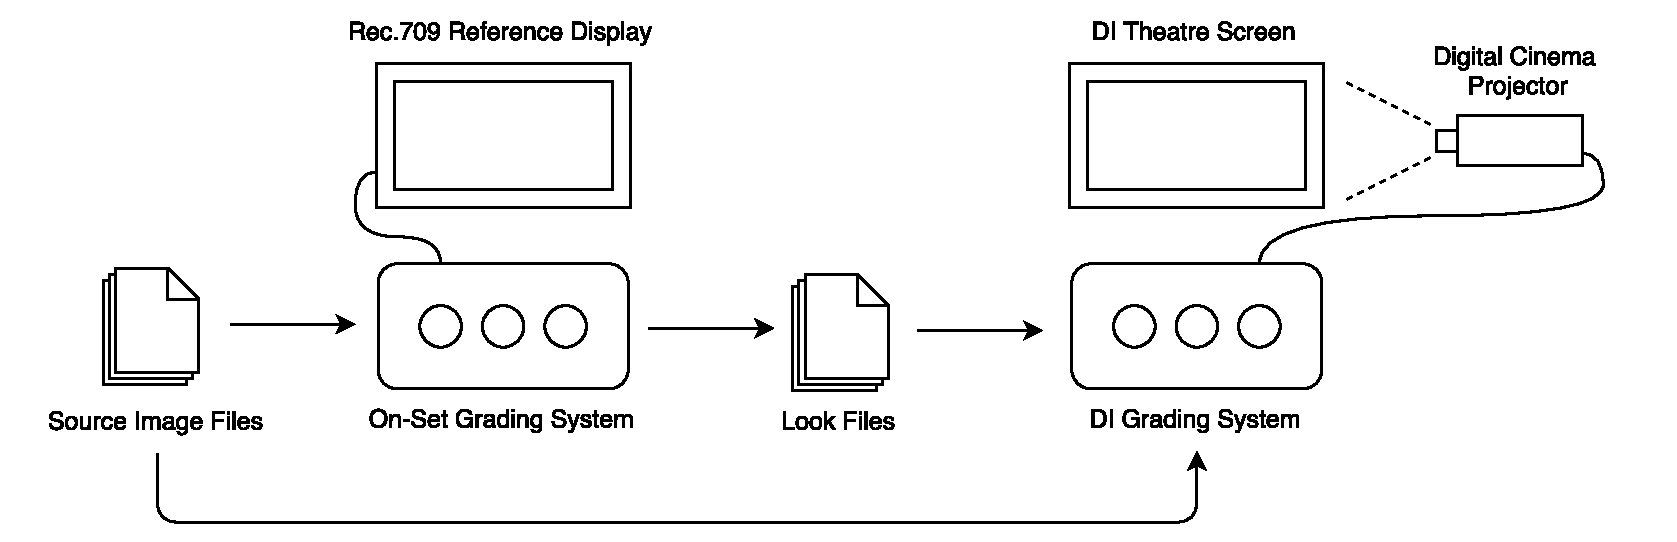
\includegraphics[width=4in]{images/workflows/workflow1.pdf}
    \caption{\small Feature Film On-Set to SDR DI Workflow}
    \label{fig:workflow1}
\end{figure*}

In this on-set to digital intermediate workflow a Rec.709 reference display is connected to the on-set grading system and a digital cinema projector is connected to the DI grading system.  In this workflow it is suggested that the on-set grading system be configured according to the Output Transform Application specified in Section \ref{sec:ot-app-rec709d60sim}.  The DI grading system should be configured according to the Output Transform Application specified in Section \ref{sec:ot-app-p3d60}, or alternatively Section \ref{sec:ot-app-p3dci}.  The recommendations are summarized in Table \ref{tab:sum-ff-os-workflow}.

\begin{table}[ht!]
\centering
\begin{tabular}{|p{0.5in}|p{1.2in}|p{3.75in}|}
\hline
\textbf{System}   & \textbf{Display}            & \textbf{Suggested ODT}                                                  \\ \hline
On-set \newline Grading & Rec.709 Reference Monitor   & \texttt{\seqsplit{ODT.Academy.Rec709\_D60sim\_100nits\_dim.a1.0.3}} \\ \hline
DI \newline Grading & P3 Digital Cinema Projector & \texttt{\seqsplit{ODT.Academy.P3D60\_48nits.a1.0.3}} \newline or \newline \texttt{\seqsplit{ODT.Academy.P3DCI\_48nits.a1.0.3}}           \\ \hline
\end{tabular}
\caption[Workflows - Feature Film (Onset-DI) - Suggested ODTs]{Summary of suggested ODTs}
\label{tab:sum-ff-os-workflow}
\end{table}

\subsubsection{Discussion}
In the On-Set to Digital Intermediate workflow, using the suggested ODT will provide a white point match between the two environments.  The displays will not match to the degree there are colors in the content that would take advantage of the P3 color space in DI since those colors could not be reproduced on-set with the Rec.709 monitor.  It's important to recognize that the colorimetry will not measure as matching due the the surround environment differences associated with the DI grading and On-set ODTs.  The On-set ODT is designed for a dim surround environment where the DI grading ODT is designed for a dark surround environment.  If viewed in their correct respective environments using the suggested ODTs should provide a visual match since the ODTs compensate for perceptual differences imposed by the viewing environments.

\subsection{Production and Mastering -- HDR On-Set and Digital Intermediate}
\subsubsection{Summary}
\subsubsection{Workflow}
\subsubsection{Discussion}

\subsection{On-set and Dailies -- iPad Review}
\subsubsection{Summary}
\subsubsection{Workflow}
\subsubsection{Discussion}

\subsection{Visual Effects}
\subsubsection{Summary}
\subsubsection{Workflow}
\subsubsection{Discussion}


\section{Episodic Television Workflows}

\subsection{Production and Mastering -- SDR On-Set and Digital Intermediate}
\subsubsection{Summary}
\subsubsection{Workflow}
\subsubsection{Discussion}

\subsection{Production and Mastering -- HDR On-Set and Digital Intermediate}
\subsubsection{Summary}
\subsubsection{Workflow}
\subsubsection{Discussion}

\subsection{On-set and Dailies -- iPad Review}
\subsubsection{Summary}
\subsubsection{Workflow}
\subsubsection{Discussion}

\subsection{Visual Effects}
\subsubsection{Summary}
\subsubsection{Workflow}
\subsubsection{Discussion}






